\documentclass[11pt]{article}

\usepackage[a4paper,margin=24mm]{geometry}
\usepackage[T1]{fontenc}
\usepackage[utf8]{inputenc}
\usepackage{lmodern}
\usepackage{microtype}
\usepackage{amsmath,amssymb}
\usepackage{booktabs}
\usepackage{tabularx}
\usepackage{array}
\usepackage{enumitem}
\usepackage{xcolor}
\usepackage{hyperref}
\usepackage{fancyhdr}
\usepackage{listings}
\usepackage{tikz}
\usetikzlibrary{arrows.meta,positioning}

\definecolor{DeepBlue}{RGB}{30,65,110}
\definecolor{SoftGray}{RGB}{245,246,248}
\definecolor{CodeGray}{RGB}{70,70,70}
\hypersetup{colorlinks=true,linkcolor=DeepBlue,urlcolor=DeepBlue,citecolor=DeepBlue}

\pagestyle{fancy}
\fancyhf{}
\lhead{Symmetry-first sampling of planar contact graphs}
\rhead{Technical note}
\cfoot{\thepage}
\setlength{\headheight}{14pt}

\setlist[itemize]{topsep=4pt,itemsep=2pt,parsep=1pt}
\setlist[enumerate]{topsep=4pt,itemsep=3pt,parsep=1pt}
\setlength{\parindent}{0pt}
\setlength{\parskip}{6pt}

\lstset{
  basicstyle=\ttfamily\small,
  backgroundcolor=\color{SoftGray},
  frame=single,
  rulecolor=\color{black!15},
  breaklines=true,
  columns=fullflexible,
  xleftmargin=4pt,
  xrightmargin=4pt,
  aboveskip=7pt,
  belowskip=7pt,
  commentstyle=\color{CodeGray}
}

\newcommand{\OUT}{\texttt{OUTSIDE}}
\newcommand{\Cq}{C_q}
\newcommand{\Dq}{D_q}

\title{\textbf{Symmetry-First Sampling of Planar Contact Graphs}\\
\large An informal design note for exhaustive-in-support, symmetry-biased exploration}
\author{}
\date{August 2026}

\begin{document}
\maketitle

\begin{abstract}
The exact geometric solver is expensive enough that the order in which candidate contact structures are explored matters. The goal of this note is to describe a sampler that gives a deliberate and substantial fraction of its budget to symmetric candidates, gives more budget to stronger symmetries than to weaker ones, and nevertheless retains complete coverage of the admissible graph space. The central construction is simple: once an action of a symmetry group on the vertices has been fixed, all invariant graphs are obtained by selecting whole \emph{edge orbits}. For cyclic rotation symmetry this reduces to a compact ``orbit plus modular shift'' representation. A randomized exhaustive traversal of that representation, combined with canonicalization, pruning, and a weighted scheduler across symmetry strata, gives both practical stochastic exploration and a precise no-missing-graphs guarantee.
\end{abstract}

{\small\tableofcontents}
\newpage

\section{Problem setting}

The program ultimately runs an exact solver on contact structures for monohedral subdivisions of a disk. Before that expensive stage, it needs a way to explore a finite range of planar contact graphs. The intended ranges of tile counts are currently
\[
N\in\{3,4,\ldots,13,18,19\}.
\]
Here \(N\) denotes the number of tiles. The contact graph also contains a distinguished vertex \OUT, representing the exterior of the disk, so the graph itself has \(N+1\) vertices.

At the graph stage, the important generic conditions are assumed to include at least:
\begin{itemize}
  \item planarity;
  \item the distinguished \OUT\ vertex;
  \item minimum degree at least three, counting \OUT\ in the same graph;
  \item any additional graph-level admissibility conditions already present in the implementation.
\end{itemize}

A further condition may be 3-connectivity. It is useful to separate two cases throughout this note:
\begin{itemize}
  \item if 3-connectivity is guaranteed, a planar graph has an essentially unique embedding on the sphere, up to reflection, and geometric symmetry testing is comparatively simple;
  \item if 3-connectivity is not guaranteed, the correct search object is really a planar \emph{map} (a graph plus a rotation system / embedding), because the same abstract graph can have inequivalent embeddings and an abstract automorphism need not preserve the embedding that matters to the tiling problem.
\end{itemize}

The sampling problem is not to sample uniformly from all admissible graphs. Uniform sampling would in fact be undesirable here: asymmetric graphs vastly outnumber highly symmetric ones. The desired prior should instead have four properties.

\begin{enumerate}
  \item \textbf{Complete support.} No admissible graph should be assigned probability zero merely because it is asymmetric or belongs to a weak symmetry class.
  \item \textbf{Explicit symmetry budget.} A significant fraction of computation should be reserved for genuinely symmetric candidates, independently of how numerous asymmetric candidates are.
  \item \textbf{Preference for strong symmetry.} Within the symmetric budget, high rotational order should receive more exploration than low order.
  \item \textbf{No omissions inside a stratum.} If, for example, the sampler explores order-three rotational symmetry, its construction must include every order-three invariant graph, including configurations with several rings, relative phase shifts between rings, and several simultaneous inter-ring contact patterns.
\end{enumerate}

The fourth point is the nontrivial one. The rest of the note is mainly about making that guarantee precise.

\section{Do not sample a graph and then reward symmetry}

A tempting design is:
\begin{quote}
Generate an admissible planar graph from a broad distribution, compute its automorphism group, and multiply its priority by a large factor if it is symmetric.
\end{quote}

This is the wrong architecture when symmetry is rare. Even a very large per-graph multiplier can be overwhelmed by the combinatorial multiplicity of asymmetric graphs. If only one candidate in a million generated by the base distribution has a useful symmetry, multiplying its score by one thousand still leaves almost all computation asymmetrical.

Instead, symmetry should be selected \emph{before} the graph is generated. The sampler should contain explicit channels such as
\begin{itemize}
  \item unrestricted / general;
  \item reflection-only candidates;
  \item candidates invariant under a rotation of order two;
  \item candidates invariant under a rotation of order three;
  \item candidates invariant under a rotation of order four;
  \item and so on for every rotational order compatible with the chosen tile count.
\end{itemize}

A scheduler then reserves a chosen fraction of the total budget for these channels. This makes the symmetry allocation independent of the relative number of asymmetric graphs in the universe.

\section{What ``rotation of order q'' means combinatorially}

Fix a desired geometric rotation of order \(q>1\). The generator of that rotation acts as a permutation of the tile vertices and fixes \OUT.

For actual tiles that are topological disks, the orbit structure is very restricted. Apart from a possible single tile fixed by the rotation, tile vertices come in complete orbits of length \(q\). The reason is worth making explicit. If a closed Jordan tile is invariant under a nontrivial rotation, Brouwer's fixed-point theorem forces the rotation center to belong to that tile. The center cannot lie on the tile's Jordan boundary: the induced finite-order orientation-preserving homeomorphism of the boundary circle would then have a fixed point, which would force that boundary action to be the identity, impossible for a nontrivial planar rotation. Hence the rotation center lies in the tile interior. Two distinct tiles with disjoint interiors therefore cannot both be invariant under a nontrivial rotation. Moreover, an orbit of intermediate size strictly between one and \(q\) would consist of several tiles, each invariant under a nontrivial subgroup and hence each containing the rotation center in its interior, which is again impossible. Thus every noncentral tile orbit has full length \(q\).

Consequently, if there are \(N\) tiles, an order-\(q\) rotation is possible only when either
\begin{itemize}
  \item \(N\) is divisible by \(q\), in which case all tiles may occur in full \(q\)-orbits; or
  \item \(N-1\) is divisible by \(q\), in which case there may be one rotation-fixed central tile and all other tiles occur in full \(q\)-orbits.
\end{itemize}

This is a useful reduction: not every integer between two and \(N\) is a possible rotational order for a fixed \(N\).

\begin{table}[ht]
\centering
\small
\begin{tabular}{c l}
\toprule
Tile count \(N\) & Possible nontrivial rotational orders \(q\) \\
\midrule
3  & 2, 3 \\
4  & 2, 3, 4 \\
5  & 2, 4, 5 \\
6  & 2, 3, 5, 6 \\
7  & 2, 3, 6, 7 \\
8  & 2, 4, 7, 8 \\
9  & 2, 3, 4, 8, 9 \\
10 & 2, 3, 5, 9, 10 \\
11 & 2, 5, 10, 11 \\
12 & 2, 3, 4, 6, 11, 12 \\
13 & 2, 3, 4, 6, 12, 13 \\
18 & 2, 3, 6, 9, 17, 18 \\
19 & 2, 3, 6, 9, 18, 19 \\
\bottomrule
\end{tabular}
\caption{Candidate rotational orders under the full-orbit plus optional central-tile model. \OUT\ is not included in \(N\).}
\end{table}

For example, with 19 tiles an order-four rotation is not possible in this model: 19 is neither a multiple of four nor one more than a multiple of four. Orders 18 and 19 are possible in principle: order 18 corresponds to one central tile plus one orbit of 18, while order 19 corresponds to one orbit of 19.

\section{The core exhaustive construction: edge orbits}

The most important idea in this note is completely general.

Suppose a finite group \(H\) acts on the vertices of a candidate graph. Consider every unordered pair of distinct vertices. The group also acts on these pairs. Therefore the possible edges split into \emph{orbits of edges} under \(H\).

An \(H\)-invariant graph cannot contain only part of such an orbit. If it contains one edge, it must contain every image of that edge under the symmetry. Conversely, any union of complete edge orbits is automatically invariant under the prescribed vertex action.

Therefore:

\begin{quote}
\textbf{For a fixed group action on the vertices, every invariant simple graph is exactly a subset of the possible edge orbits.}
\end{quote}

This is the exhaustiveness guarantee. It is not a heuristic statement. If the edge-orbit catalog is complete, an invariant graph cannot be omitted: its edge set is necessarily one of the subsets represented by the search tree.

The generic generator is consequently:

\begin{lstlisting}
input: vertex set V, group action H on V

pair_orbits = orbits of unordered pairs {u,v}, u != v, under H

search(partial_selection):
    choose one undecided pair_orbit E
    recurse with E excluded
    recurse with E included

at a leaf:
    the union of selected pair_orbits is one H-invariant graph
\end{lstlisting}

In practice, almost all branches are cut long before reaching a leaf by planarity, degree, connectivity, and canonicality tests.

\section{Specialization to cyclic rotations: rings and modular shifts}

For rotations, the generic pair-orbit construction has a much more transparent representation.

Suppose there are \(a\) full tile orbits under an order-\(q\) rotation. Name them
\[
A^{(1)}, A^{(2)}, \ldots, A^{(a)}.
\]
Within one orbit, write
\[
A^{(r)}_0,A^{(r)}_1,\ldots,A^{(r)}_{q-1},
\]
with the rotation sending index \(i\) to \(i+1\) modulo \(q\).

There may additionally be a central fixed tile \(C\), and \OUT\ is always fixed.

\subsection{Edges between two different tile orbits}

Take two distinct orbits \(A\) and \(B\). For every modular shift \(d\in\{0,\ldots,q-1\}\), there is an edge orbit
\[
E(A,B;d)=\bigl\{A_i B_{i+d}: i\in\mathbb Z/q\mathbb Z\bigr\}.
\]

Thus there are \(q\) fundamentally different relative alignments between two \(q\)-orbits. Selecting shift zero connects aligned members; selecting shift one connects each member to the next member of the other ring; selecting several shifts at once gives several simultaneous contact patterns.

This is exactly what is needed to avoid missing ``misaligned ring'' examples.

For example, with order three:
\begin{lstlisting}
A-B shift 0:
    A0--B0, A1--B1, A2--B2

A-B shift 1:
    A0--B1, A1--B2, A2--B0

A-B shift 2:
    A0--B2, A1--B0, A2--B1
\end{lstlisting}

If a middle ring must touch both the aligned and the following tiles of an inner ring, the generator simply selects both shift zero and shift one. Nothing in the representation forces a single alignment.

\subsection{Edges inside one tile orbit}

Inside a single orbit \(A\), possible edge orbits are indexed by an offset
\[
d=1,2,\ldots,\left\lfloor\frac q2\right\rfloor.
\]
Offset \(d\) represents the edges between \(A_i\) and \(A_{i+d}\). Offsets \(d\) and \(q-d\) are the same undirected edge orbit.

The usual ring is simply offset one. Longer chords in the orbit correspond to larger offsets.

There is one small implementation detail worth keeping: when \(q\) is even and \(d=q/2\), the edge orbit has only \(q/2\) distinct edges, and selecting it increases the degree of each orbit vertex by one. For other internal offsets, the edge orbit has \(q\) edges and increases the degree of every orbit vertex by two.

\subsection{Edges to fixed vertices}

For every full tile orbit \(A\), there is one possible orbit of edges to \OUT:
\[
\{\OUT A_i : i=0,\ldots,q-1\}.
\]

If a central fixed tile \(C\) exists, there is similarly one possible edge orbit
\[
\{C A_i : i=0,\ldots,q-1\}.
\]

Finally, an edge between \(C\) and \OUT\ is a single fixed edge and must also be allowed if it is meaningful in the graph model.

\subsection{The three-ring example}

Consider nine tiles with order-three rotation. Let the three tile orbits be
\begin{lstlisting}
OUTER  = A0 A1 A2
MIDDLE = B0 B1 B2
INNER  = C0 C1 C2
\end{lstlisting}

A candidate with three rings, aligned outer-to-middle contacts, and shifted middle-to-inner contacts is represented by the Boolean choices
\begin{lstlisting}
within A, offset 1 = true
within B, offset 1 = true
within C, offset 1 = true

A-B shift 0 = true
B-C shift 1 = true
\end{lstlisting}

If every middle tile is to touch two members of the inner ring, use
\begin{lstlisting}
B-C shift 0 = true
B-C shift 1 = true
\end{lstlisting}

Hence the modular-shift model explicitly contains the examples that are easy to lose in a naive ``draw one sector and repeat it'' construction.

\section{A quotient / voltage-graph viewpoint}

It is often convenient to think of the rotational representation as a quotient graph.

Each full orbit of \(q\) tiles becomes one quotient vertex. An inter-orbit contact carries a label \(d\) modulo \(q\), meaning that copy \(i\) of the first orbit connects to copy \(i+d\) of the second. Several differently labeled quotient edges may coexist between the same quotient vertices because they lift to different sets of edges in the full simple graph.

This is essentially a cyclic voltage-graph representation. It is useful for implementation because the search state is small even when the lifted graph has 18 or 19 tile vertices. The full graph is expanded only when a planarity or final validation routine needs it.

The quotient should not be confused with an ordinary planar quotient drawing. The full lifted graph is the object whose planarity matters; the modular labels carry information that a plain quotient multigraph would lose.

\section{How large is the raw Boolean search?}

For \(a\) full \(q\)-orbits with no central tile, the number of basic edge-orbit variables is approximately
\[
q\binom a2 + a\left\lfloor\frac q2\right\rfloor + a,
\]
where the three terms are, respectively, inter-orbit shifts, internal offsets, and contacts to \OUT.

With a central tile, add another \(a\) variables for central-to-orbit contacts and one possible central-to-\OUT\ edge.

The raw power set can still be large. For example, six order-three tile orbits already give dozens of Boolean variables. Therefore exhaustive edge-orbit generation is useful only together with strong incremental pruning. Fortunately, the target graphs are tiny in absolute size, so graph tests can be run very aggressively.

\section{Incremental pruning}

The generator should be implemented as a constraint search rather than as ``enumerate every subset and test at the end.''

\subsection{Planarity}

Planarity gives the most important monotone cut. Once the currently selected edge orbits produce a nonplanar graph, adding more edges can never restore planarity. Therefore the entire branch is dead.

\begin{lstlisting}
include edge orbit E
expand or update the partial graph
if partial graph is nonplanar:
    prune this branch permanently
\end{lstlisting}

At fewer than twenty tile vertices, even rebuilding and retesting the graph from scratch is cheap enough for a first implementation. Incremental planarity can be added only if profiling later justifies it.

\subsection{Planar edge-count bound}

For a simple planar graph with at least three vertices, the usual edge-count bound gives an extremely cheap preliminary check. Since an edge-orbit decision may add \(q\) edges at once, this catches some branches before a full planarity call.

\subsection{Minimum degree feasibility}

For each vertex orbit, maintain two values:
\begin{itemize}
  \item its current degree after the selected edge orbits;
  \item the maximum degree it could still reach if every relevant undecided orbit were selected.
\end{itemize}

If the second value is below the required minimum degree, the branch can never be completed and should be pruned immediately.

Because symmetry makes all vertices in a full orbit equivalent, this check is naturally performed once per orbit rather than once per vertex.

\subsection{Connectivity feasibility}

Build an optimistic graph containing both selected and still-available edges. If even this optimistic graph cannot become connected, the branch is dead.

If 3-connectivity is a genuine requirement, the same idea can be used as a necessary test: if the optimistic completion graph already has vertex connectivity below three, no subgraph of it can become 3-connected. A cheaper implementation can defer the exact 3-connectivity test until complete candidates and add this stronger pruning later.

\subsection{Other domain-specific cuts}

Any exact graph-level constraint already known to the program should be inserted here. The search is especially effective when inexpensive conditions are evaluated before expensive ones.

A reasonable initial order is:
\begin{enumerate}
  \item simple arithmetic bounds;
  \item degree feasibility;
  \item connectivity feasibility;
  \item planarity;
  \item domain-specific structural constraints;
  \item full connectivity / 3-connectivity checks at leaves.
\end{enumerate}

\section{Choosing the next edge orbit}

A fixed arbitrary variable order is rarely optimal. At each partial state, prefer decisions that are likely to create an early contradiction.

Useful heuristics include selecting an undecided edge orbit that:
\begin{itemize}
  \item touches a vertex orbit that is still below minimum degree;
  \item joins currently separate components;
  \item adds many lifted edges and is therefore likely to violate planarity;
  \item interacts with already dense parts of the partial graph;
  \item has high impact on the current symmetry quotient.
\end{itemize}

This is ordinary constraint-programming logic: force the difficult choices early so that impossible branches die close to the root.

For stochastic exploration, the heuristic need not be deterministic. One can choose randomly among the few highest-scoring undecided variables.

\section{From exhaustive enumeration to stochastic sampling}

The same search tree supports two different operating modes.

\subsection{Mode A: randomized exhaustive streams}

This is the strongest option when the finite search is manageable.

For each symmetry action, run an exhaustive depth-first or best-first generator, but randomize the order in which sibling branches are traversed. The branch order can be generated from a reproducible pseudorandom hash of
\begin{itemize}
  \item a global seed;
  \item the symmetry stratum;
  \item a canonical encoding of the partial state.
\end{itemize}

The output order then looks stochastic, but every surviving leaf is eventually visited exactly as in ordinary enumeration. This gives a much stronger guarantee than saying merely that every graph has positive sampling probability.

A persistent generator for each stratum can be paused after yielding one candidate and resumed later. A global scheduler decides which generator receives the next unit of computation.

\subsection{Mode B: restart-based Monte Carlo}

If exhaustive streams are too large, use randomized constructive runs. At every undecided edge orbit, choose include or exclude with probabilities strictly between zero and one, modified by the current graph density and feasibility heuristics. Backtrack when a contradiction is reached.

As long as every admissible decision retains positive probability, every graph represented by the action retains positive probability of being generated. This gives complete \emph{support}, but not finite-time coverage and not anything close to uniformity.

For the present application, Mode A is preferable wherever possible because it naturally avoids repeated sampling of the same branch and provides eventual exhaustive coverage. Mode B is a useful fallback or a way to obtain very fast exploratory runs.

\section{Symmetry strata and maximal symmetry}

A candidate generated under an order-three action may secretly have order six. Likewise, a graph generated under a pure cyclic action may also admit a reflection and therefore have dihedral symmetry.

For ranking and accounting, the candidate should therefore be classified \emph{after} generation by its actual maximal geometric symmetry.

Useful disjoint output strata are:
\begin{itemize}
  \item asymmetric;
  \item reflection symmetry but no nontrivial rotation;
  \item maximal rotation order \(q\), no compatible reflection;
  \item maximal rotation order \(q\), with a compatible reflection (dihedral type).
\end{itemize}

The generation source and the final stratum are not necessarily the same. This is not a problem. A candidate produced by the order-three generator and discovered to have order six should be routed to the order-six pool and counted against the order-six coverage target.

This post-classification prevents stronger-symmetry graphs from being accidentally counted many times as representatives of all of their weaker subgroups.

\section{Geometric symmetry versus abstract graph automorphism}

Edge-orbit generation guarantees an abstract graph automorphism. For the disk problem, one needs the corresponding symmetry to be compatible with a planar embedding.

If the graph is 3-connected, Whitney's uniqueness theorem gives an essentially unique embedding on the sphere. An automorphism can then be classified as orientation-preserving or orientation-reversing by how it acts on the cyclic orders around vertices. An intended rotation must be orientation-preserving; an intended mirror reflection must be orientation-reversing.

This distinction is especially important for order two: the same abstract permutation type can represent either a half-turn or a reflection, and the embedding determines which geometric interpretation is valid.

If the graph is not known to be 3-connected, checking one arbitrary planar embedding is not sufficient. In that case there are two safe approaches:
\begin{enumerate}
  \item promote the search object from an abstract graph to a combinatorial planar map and generate/map-test symmetries directly on darts and cyclic orders; or
  \item use an embedding-aware decomposition, for example an SPQR-based treatment, to decide whether some planar embedding realizes the prescribed automorphism.
\end{enumerate}

For the current small sizes, proving or enforcing 3-connectivity upstream would simplify the entire symmetry pipeline considerably.

\section{Canonicalization and duplicate control}

The orbit representation itself is labeled. Renaming orbit families, shifting the phase of one orbit, reversing all modular indices, or using a weaker subgroup of a stronger symmetry can lead to multiple descriptions of the same graph.

The simplest robust implementation is therefore:
\begin{enumerate}
  \item construct a complete candidate;
  \item color \OUT\ as a distinguished vertex;
  \item compute a canonical labeling of the graph, or of the planar map if the embedding is part of the state;
  \item use the canonical encoding as a hash key;
  \item discard candidates whose key has already been seen;
  \item compute the actual symmetry group and route the candidate to its maximal stratum.
\end{enumerate}

For the present vertex counts, this straightforward ``generate, canonicalize, hash'' approach is the correct first implementation unless measurements show otherwise.

If the search eventually becomes so large that storing all previous canonical keys is undesirable, the standard upgrade is a \emph{canonical construction path}: only augmentations that are canonical relative to the child object are accepted. This is the general isomorph-free generation strategy associated with McKay and used in highly optimized graph generators such as \texttt{plantri}. It avoids global duplicate storage but is substantially more delicate to implement correctly.

\section{Reflection-only symmetry}

Reflection symmetry is handled by the same edge-orbit principle.

For an involutive reflection action, tile vertices split into:
\begin{itemize}
  \item fixed vertices, corresponding to tiles invariant under the reflection;
  \item swapped pairs of vertices.
\end{itemize}

Unlike nontrivial rotations, a reflection can fix several different tiles arranged along its axis, so the number of fixed tile vertices is not restricted to zero or one. For a given tile count \(N\), enumerate every possible number \(f\) of fixed tile vertices having the same parity as \(N\); the remaining \(N-f\) vertices form \((N-f)/2\) swapped pairs.

For each such involution, form all orbits of unordered vertex pairs and run the same subset search with the same pruning rules.

For dihedral symmetry, a separate direct generator is not strictly necessary. Every dihedrally symmetric graph already has the corresponding cyclic rotation, so the cyclic generators can produce it and the final automorphism analysis can detect the additional reflection. Direct dihedral generation can be added later if it gives a useful speedup.

\section{The global scheduler}

The symmetry generators solve the within-stratum problem. A separate scheduler decides how often each stratum is explored.

The scheduler should not infer the symmetry budget from the number of available graphs. It should impose it explicitly. A practical decomposition is
\[
P = p_{\mathrm{general}} P_{\mathrm{general}} + p_{\mathrm{sym}} P_{\mathrm{sym}},
\qquad p_{\mathrm{general}}+p_{\mathrm{sym}}=1.
\]

For example, one might begin with 30 percent of the budget assigned to an unrestricted complete-support generator and 70 percent to explicit symmetry strata. The precise numbers are tuning parameters, not mathematical requirements.

Inside the symmetric budget, give a stratum \(s\) with rotational order \(q_s\) a base weight such as
\[
w_s = q_s^{\alpha} b_s,
\]
where \(\alpha>0\) controls how aggressively stronger rotations are preferred and \(b_s\) can give a modest extra factor to dihedral symmetry.

A quadratic choice \(\alpha=2\) is a reasonable starting point: order six then receives nine times the rotational weight of order two before coverage corrections.

However, pure proportional weighting is not sufficient because weak or rare strata can be starved. Use a floor-plus-preference mixture:
\[
P(s\mid\mathrm{sym}) =
\varepsilon\frac{1}{|S|}
+(1-\varepsilon)\frac{w_s}{\sum_{t\in S}w_t}.
\]

The uniform floor ensures that every active stratum continues to receive work. The weighted term makes strong symmetries substantially more common.

\section{Coverage first, weighting second}

If the practical objective is ``within a few thousand candidates, make sure every nontrivial symmetry class has actually been explored,'' relying on random probabilities is unnecessary.

Use an explicit coverage phase.

For every potentially nonempty stratum, assign a small target number of \emph{unique} candidates. The scheduler first services strata with the largest deficit relative to their target. Once all nonempty strata have reached their minimum target, switch to the long-run weighted policy.

A useful variant is to make the target itself increase with symmetry order, for example
\[
K_s = K_0 + K_1 q_s^{\alpha}.
\]
Then high-order symmetries receive more candidates even during the initial coverage phase, while every low-order symmetry still receives a guaranteed minimum.

If a stratum generator exhausts all of its candidates before reaching the requested quota, mark it exhausted and redistribute the unused budget. This is valuable information: the generator has proved that the stratum contains fewer admissible graphs than the requested sample size, or none at all.

\section{A weighted-fair scheduling rule}

A deterministic deficit scheduler is often preferable to repeated independent random draws because it gives stronger finite-time behavior.

Maintain, for each active stratum \(s\):
\begin{itemize}
  \item a target long-run weight \(w_s\);
  \item the amount of work already allocated \(a_s\);
  \item optionally a coverage target \(K_s\) and the number of unique candidates already obtained.
\end{itemize}

At each step, choose the stratum with the largest normalized deficit relative to where it should be under its target share, with a strong temporary bonus for unmet coverage quotas. Add small random tie-breaking noise if a stochastic order is desired.

This behaves like weighted fair queuing: no stratum with positive weight is starved, but stronger symmetries receive more service in the long run.

\section{Ensuring complete coverage of the whole graph space}

Symmetry-first generation does not by itself cover asymmetric graphs. Therefore retain an unrestricted branch with nonzero budget.

There are two corresponding guarantees.

\subsection{Enumeration guarantee}

If the unrestricted branch is itself an isomorph-free exhaustive generator, and the scheduler is fair in the sense that every nonexhausted stream is resumed infinitely often, then every admissible graph in the finite target range is eventually visited. Symmetry streams merely change the order and dramatically accelerate access to rare symmetric candidates.

\subsection{Monte Carlo support guarantee}

If the unrestricted branch is a randomized constructive sampler rather than an enumerator, require every admissible local decision to retain positive probability. Then every admissible graph has nonzero probability of being generated. In an ideal infinite run it is eventually observed with probability one under the usual independent/recurrent sampling assumptions, but there is no practical finite-time coverage guarantee.

For this reason, a randomized exhaustive stream is preferable whenever the underlying enumerator is available.

\section{A practical hybrid architecture}

A robust first implementation can be organized into four layers.

\subsection*{Layer 1: source generators}

Maintain generators for:
\begin{itemize}
  \item one unrestricted admissible-graph stream;
  \item each allowed cyclic action \((N,q)\);
  \item each reflection action \((N,f)\), where \(f\) is the number of fixed tile vertices.
\end{itemize}

Each symmetry generator uses edge orbits and incremental pruning.

\subsection*{Layer 2: canonical output}

Every produced candidate is canonicalized globally. Duplicates are discarded regardless of which source generated them.

\subsection*{Layer 3: actual symmetry classification}

Compute the maximal embedding-compatible symmetry fixing \OUT. Route the candidate to its true output stratum: asymmetric, reflection-only, maximal cyclic order \(q\), or maximal dihedral order \(q\).

\subsection*{Layer 4: scheduler}

Initially pursue explicit coverage quotas. Afterwards allocate a fixed general budget and a symmetry budget, with symmetry weights increasing with rotational order.

A schematic loop is:

\begin{lstlisting}
while search_budget_remains:
    source = scheduler.choose_source()
    candidate = source.next_candidate()

    if source.exhausted:
        scheduler.disable(source)
        continue

    key = canonical_key(candidate)
    if key in global_seen:
        continue
    global_seen.add(key)

    symmetry = classify_maximal_map_symmetry(candidate, OUTSIDE)
    stratum = route(symmetry)
    statistics[stratum].record(candidate)

    exact_solver_queue.push(candidate, priority=stratum_priority(stratum))
\end{lstlisting}

The generator scheduler and the exact-solver queue need not use the same priority. For example, the generator may aggressively cover all symmetry strata while the solver queue additionally uses geometric or machine-learned promise scores.

\section{Why this construction cannot forget a shifted multi-ring graph}

The exhaustiveness argument is worth stating explicitly because it is the main reason to use this design.

Fix an order-\(q\) action on the tile vertices. Let \(G\) be any simple graph invariant under that action. Pick any edge of \(G\). Applying the rotation repeatedly generates the full edge orbit containing that edge. Since \(G\) is invariant, every edge in that orbit is also in \(G\). Repeating this operation for all edges partitions the complete edge set of \(G\) into edge orbits.

The generator lists every possible edge orbit, including every modular shift between every pair of tile orbits. Hence the edge set of \(G\) corresponds to one Boolean selection in the generator's search tree.

Planarity and degree pruning do not invalidate this argument: they remove only partial branches that provably cannot be completed into an admissible graph. Therefore an admissible invariant graph cannot be pruned before its leaf is reached.

The only remaining source of accidental omission would be an incorrect canonicalization or an incorrect assumption about the vertex action. This is why those two components should be unit-tested separately.

\section{Implementation details worth testing explicitly}

\subsection{Action-level unit tests}

For small \(q\), construct known examples by hand and verify that their edge-orbit encodings are generated:
\begin{itemize}
  \item one ring;
  \item two aligned rings;
  \item two rings shifted by every possible modular phase;
  \item two rings with several simultaneous shifts;
  \item three rings with different shifts on successive interfaces;
  \item a fixed central tile plus one or more rings;
  \item examples with stronger accidental symmetry than the prescribed source action.
\end{itemize}

\subsection{Exhaustiveness cross-check at small N}

For small tile counts where full planar-graph enumeration is cheap, independently enumerate every admissible graph, classify its automorphism group, and compare the symmetric subset against the symmetry-first generator. This is the strongest practical regression test for the no-omissions claim.

\subsection{Embedding checks}

If 3-connectivity is assumed, assert it in the generator and test orientation preservation/reversal of the prescribed automorphism. If it is not assumed, add explicit map-level tests before relying on symmetry classification.

\subsection{Reproducibility}

Randomized branch ordering should be seedable. Store the seed, source-stratum identifier, and canonical candidate hash so that any discovered structure can be reproduced exactly.

\section{Possible use of plantri and canonical-generation software}

Before implementing a complete unrestricted planar-graph generator from scratch, it is worth evaluating \texttt{plantri} as a source or validation oracle. It is designed for isomorph-free generation of several classes of planar graphs and can handle minimum-degree and connectivity restrictions in relevant families. Its documentation also distinguishes orientation-preserving and orientation-reversing automorphisms of planar maps.

Even if the final production sampler uses the custom edge-orbit construction, an independent generator is extremely useful for small-\(N\) cross-checks: generate the full admissible set, classify all symmetries, and verify that every symmetric object appears in the custom generator.

If the contact representation eventually permits multiple graph edges between the same pair of tile vertices, the simple-graph pair-orbit construction must be generalized to a map/dart representation. The group-orbit principle remains valid, but the atomic objects are then edge instances or darts rather than unordered vertex pairs.

\section{Recommended first version}

For the current range of fewer than twenty tiles, a deliberately simple implementation is likely sufficient.

\begin{enumerate}
  \item \textbf{Confirm the exact graph class.} In particular, confirm simple versus multigraph and whether 3-connectivity is guaranteed.
  \item \textbf{Implement cyclic actions.} For each allowed \((N,q)\), build the full-orbit representation, optional central tile, and complete modular-shift edge-orbit catalog.
  \item \textbf{Use randomized exhaustive DFS.} Include strong planarity and degree pruning, but keep the first implementation conceptually simple.
  \item \textbf{Canonicalize complete candidates.} Distinguish \OUT\ by vertex color and use a global seen set.
  \item \textbf{Classify actual maximal symmetry.} Do not assume that the generation action is maximal.
  \item \textbf{Add reflection generators.} Enumerate involution types by number of fixed tile vertices and use generic pair orbits.
  \item \textbf{Add an unrestricted stream.} This provides complete coverage outside the symmetry-focused part of the search.
  \item \textbf{Use a coverage-first scheduler.} Guarantee a minimum number of unique candidates per nontrivial symmetry stratum, with larger targets for larger \(q\).
  \item \textbf{Then switch to weighted fair sampling.} Reserve a fixed fraction of budget for the unrestricted stream and distribute the symmetric fraction with weights growing approximately like \(q^2\) or another tunable power.
  \item \textbf{Cross-check exhaustiveness at small N.} Compare against an independent planar-graph enumerator before trusting the large runs.
\end{enumerate}

This version already satisfies the essential design requirements: explicit control of the symmetry budget, preferential treatment of strong symmetry, complete support for all admissible graphs, and a constructive proof that no graph is omitted inside a prescribed symmetry action.

\section{Conceptual summary}

The central mistake to avoid is treating symmetry as a rare property discovered after sampling. Symmetry should instead be a \emph{coordinate system for generation}.

For a fixed action, the vertices are organized into symmetry orbits. The possible edges are then organized into edge orbits. Selecting complete edge orbits generates every invariant graph. For rotations, the edge orbits are simply modular shifts between tile orbits, which naturally encode aligned rings, misaligned rings, and multiple simultaneous contact patterns.

A symmetry-stratified scheduler can then reserve a large, explicit fraction of the search budget for nontrivial symmetry and bias that budget toward high rotational orders. Randomized exhaustive traversal gives stochastic-looking exploration without sacrificing eventual coverage. A separate unrestricted stream guarantees that asymmetric candidates are not excluded. Canonicalization and post-generation symmetry classification turn the overlapping source generators into disjoint maximal-symmetry output strata.

In short, the proposed search architecture is:

\begin{center}
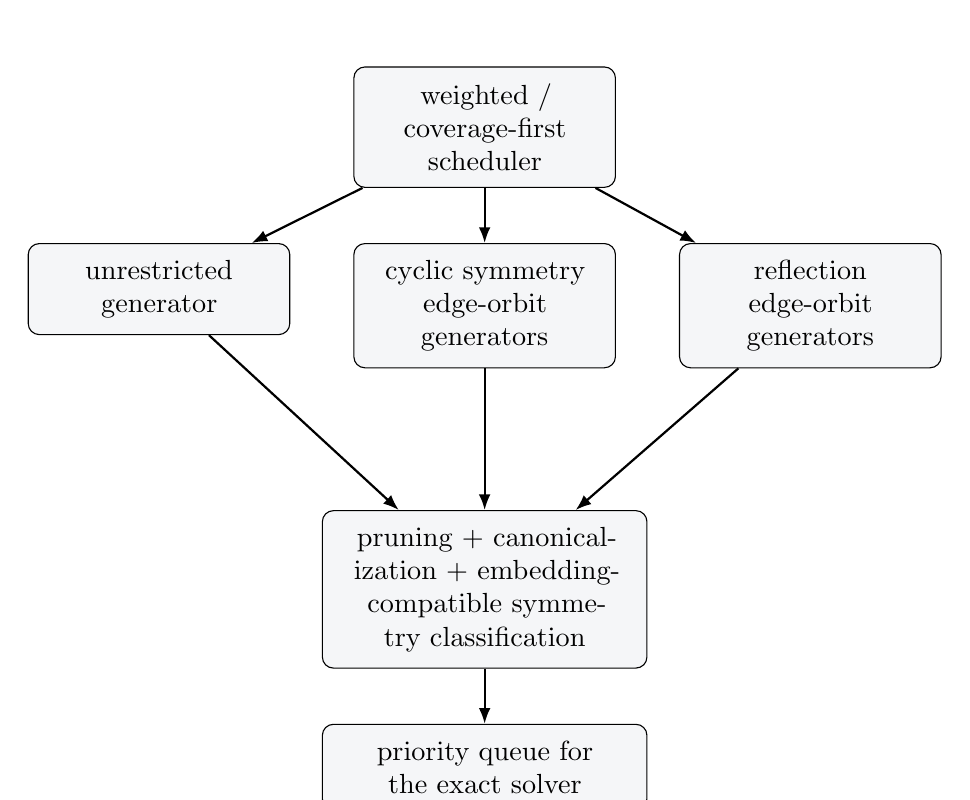
\begin{tikzpicture}[
  node distance=7mm and 8mm,
  box/.style={draw,rounded corners,align=center,fill=SoftGray,inner sep=6pt,text width=29mm},
  arr/.style={-{Latex[length=2mm]},thick}
]
\node[box] (sched) {weighted / coverage-first scheduler};
\node[box,below left=of sched] (general) {unrestricted\\generator};
\node[box,below=of sched] (cyclic) {cyclic symmetry\\edge-orbit generators};
\node[box,below right=of sched] (refl) {reflection\\edge-orbit generators};
\node[box,below=18mm of cyclic,text width=37mm] (canon) {pruning + canonicalization + embedding-compatible symmetry classification};
\node[box,below=of canon,text width=37mm] (queue) {priority queue for the exact solver};
\draw[arr] (sched) -- (general);
\draw[arr] (sched) -- (cyclic);
\draw[arr] (sched) -- (refl);
\draw[arr] (general) -- (canon);
\draw[arr] (cyclic) -- (canon);
\draw[arr] (refl) -- (canon);
\draw[arr] (canon) -- (queue);
\end{tikzpicture}
\end{center}

The important mathematical guarantee is local and simple: \emph{for a prescribed symmetry action, an invariant graph is a union of edge orbits}. Everything else---pruning, randomization, fairness, canonicalization, and ranking---can be engineered around that fact.

\section*{References and implementation pointers}
\addcontentsline{toc}{section}{References and implementation pointers}

\begin{itemize}
  \item B. D. McKay, ``Isomorph-free exhaustive generation,'' \emph{Journal of Algorithms} 26 (1998), 306--324. The canonical construction path method is the standard conceptual reference for exhaustive generation without duplicate isomorphs.
  \item G. Brinkmann and B. D. McKay, \texttt{plantri} and its user guide: \url{https://users.cecs.anu.edu.au/~bdm/plantri/}. Useful both as an independent planar-graph generator and for its treatment of automorphisms of embedded planar graphs.
  \item H. Whitney's uniqueness theorem for 3-connected planar graphs underlies the simplification that, in the 3-connected case, the planar embedding is unique up to reflection. This is the reason abstract automorphisms can then be classified cleanly as orientation-preserving or orientation-reversing map symmetries.
  \item The modular-shift quotient used here is closely related to the classical language of cyclic voltage graphs and graph coverings. That language may be useful if the rotational generator is later generalized or optimized.
\end{itemize}

\end{document}
